%----------------------------------------
% Preamble to set up the document
%----------------------------------------
\documentclass{article}

% set up packages (you shouldn't need to touch this)
\usepackage{graphicx}  % required to insert images
\usepackage{hyperref}  % for hyperlinks
\usepackage[svgnames]{xcolor}  % to change hyperlink colors
\colorlet{linkcolour}{DarkBlue}
\hypersetup{colorlinks=true, linkcolor=linkcolour, citecolor=linkcolour, urlcolor=linkcolour,}

% Margins
\topmargin=-0.45in
\evensidemargin=0in
\oddsidemargin=0in
\textwidth=6.5in
\textheight=9.0in
\headsep=0.25in

% use a sans serif font
\renewcommand{\familydefault}{\sfdefault}

%----------------------------------------
% Step 1: Edit the lecture title
%----------------------------------------
\title{
Lecture 12: Causation and Natural Experiments \\  % Lecture title
Modeling Social Data, Spring 2017 \\   % Course title
Columbia University                    % School
}

%----------------------------------------
% Step 2: Edit your name and the date
%----------------------------------------
\author{Cecilia Simas}                     % Scribe's name
\date{April 21, 2017}                % Lecture date

\begin{document}

\maketitle


%----------------------------------------
% Step 3:
% Rename uni.tex to match your uni,
% edit the filename accordingly below,
% and put your notes in this file
%----------------------------------------
\section{Random Experiments}

\subsection{Confounds}

Reviewing the example from last lecture, if we want to assess the effect of going to hospitals on health, we need to account for confounds. The cause and effect of the outcome may be affected (confounded) by a common cause, and this impacts the result. As seen in Figure 1, a person's health today has an effect on both on whether they go to hospital and their health tomorrow,

\begin{figure}[ht]
  \begin{center}
    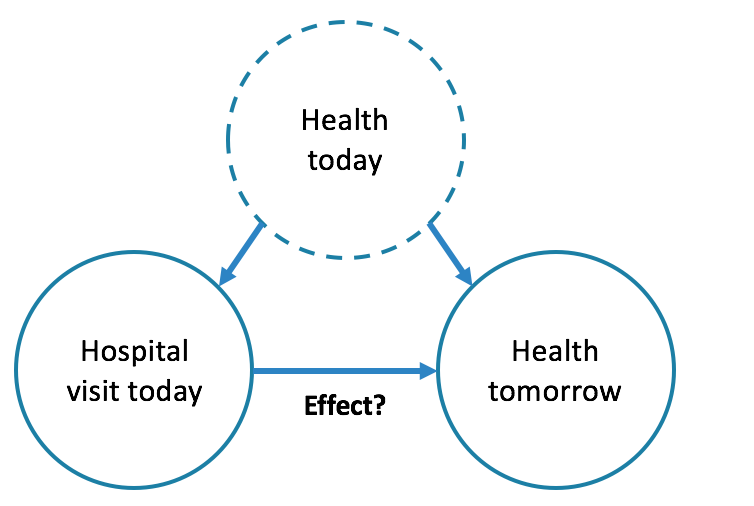
\includegraphics[width=0.3\textwidth]{figures/f1}
        \caption{ \textit{ Source: Lecture 11}}
    \label{figure 1}
  \end{center}
\end{figure}

\subsection{Random Assignment}

\textbf{Random Assignment} is the process of assigning human participants into different groups using randomization.

Using random assignment breaks the link between confounds and the results. By assigning different treatments randomly, we can account for the confounds.

For example, if the people who would go to the hospital were chosen by a coin flip, we would be able to isolate the effect of going to the hospital without the confounds, as shown in Figure 2.

\begin{figure}[ht]
  \begin{center}
    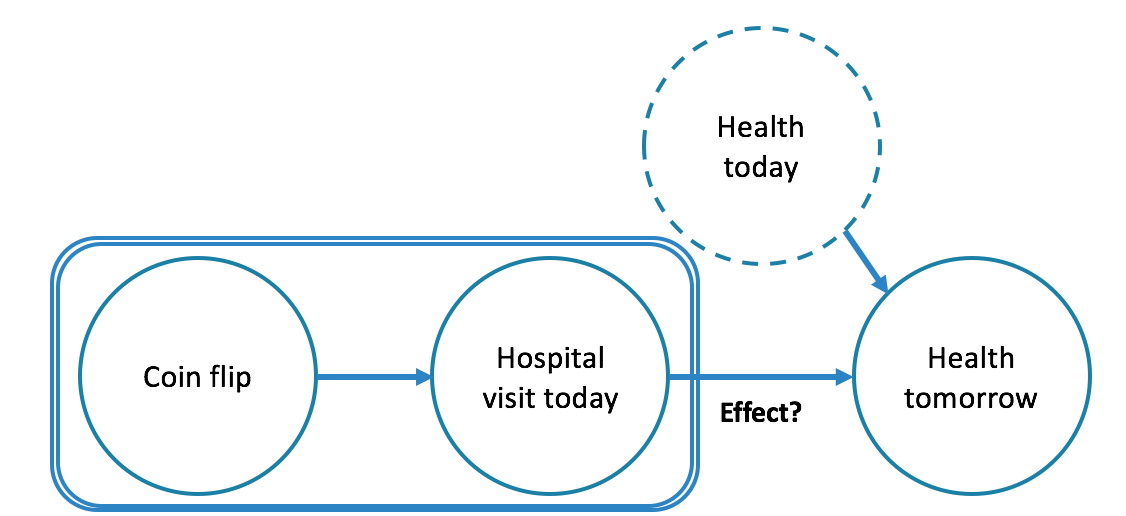
\includegraphics[width=0.3\textwidth]{figures/f2}
        \caption{ \textit{ Source: Lecture 11}}
    \label{figure 2}
  \end{center}
\end{figure}

\subsubsection{Problems with Random Assignment}

While it is considered a "gold standard" of causal inference, it may be misleading. There are 4 main issues with random assignment: small sample sizes, researcher degrees of freedom, publication bias, and p-hacking.
\subparagraph{Small sample sizes} make the sample more subject to statistical variation, leading to the potential of observing several flukes. $\alpha$, the significance level, and Power ($1-\beta$), the chance of detecting a real effect if one exists, also have an effect on the experiment. To choose these values for an experiment, it is often useful to run a \textbf{pilot study}, a smaller, preliminary version of the experiment.
\subparagraph{Researcher degrees of Freedom} may affect the results, as the flexibility in analysis is greater than the flexibility in the data. A researcher may have decided to run a different test on different data, for example, and they may also decide when to stop collecting samples such that the data fits a desired result.
\subparagraph{Publication bias}
\subparagraph{p-hacking}

\subsubsection{Other Limitations}
\begin{itemize}
\item Randomization often is possible or ethical
\item Experiments are expensive (in terms of both time and money)
\item It may be difficult to create feasible parallel worlds
\item People may be non-compliers: they may not follow the rules of the test
\end{itemize}

\subsubsection{Measuring Compliance Rates}
To measure compliance rates, measure the fraction of people that accept treatment in the treatment group, and the fraction that gets treated anyway in the control group.

\subsection{Counterfactuals}

\textbf{Counterfactuals} are events or outcomes that did not happen, "what if?" questions. However, to isolate causal effect, we have to change one and only one thing and compare outcomes, so we are not able to see the counterfactual.

\section{Natural Experiments}

Sometimes, experiments happen naturally, without needing to be formally designed. There are four main kinds of Natural Experiment: as-if random, instrumental variables, discontinuities, and difference in differences.

\subsection{As-if Random}
\subparagraph{Nature randomly assigns conditions, and people comply} An example of this is the Cholera outbreak in London in 1854, in which people were exposed to different water sources.

\subsection{Instrumental Variables}
\subparagraph{An instrument independently shifts the distribution of the treatment} For example, a lottery determines the military draft. It functions like a random assignment, and helps obtain results.

\begin{figure}[ht]
  \begin{center}
    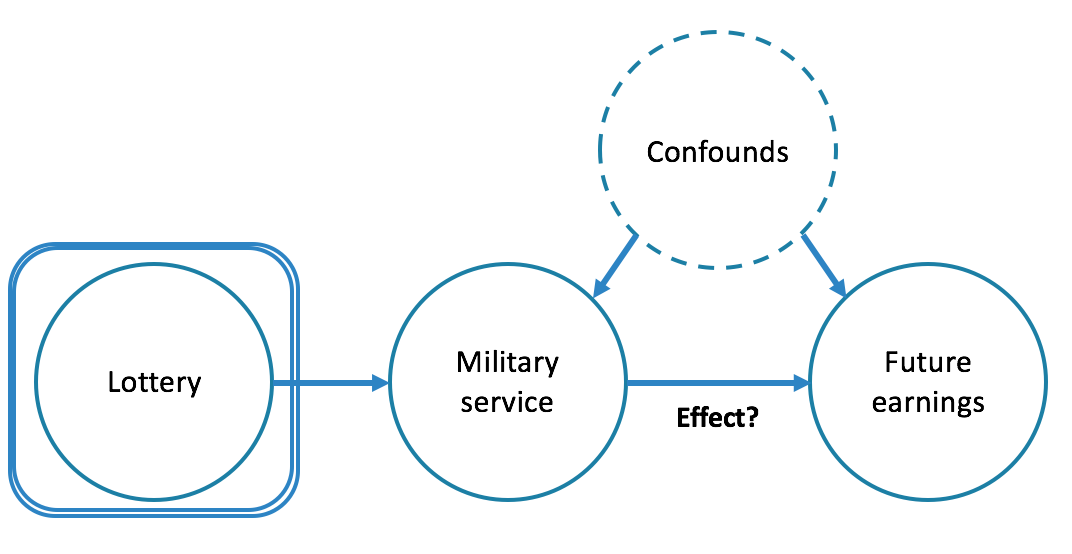
\includegraphics[width=0.3\textwidth]{figures/f3}
        \caption{ \textit{ Source: Lecture 11}}
    \label{figure 3}
  \end{center}
\end{figure}


\subsection{Regression Discontinuities}
\subparagraph{Things change around an arbitrarily chosen threshold} Yelp reviews, for example, round the stars arbitrarily, resulting in the discontinuity seen in Figure 4.

\begin{figure}[ht]
  \begin{center}
    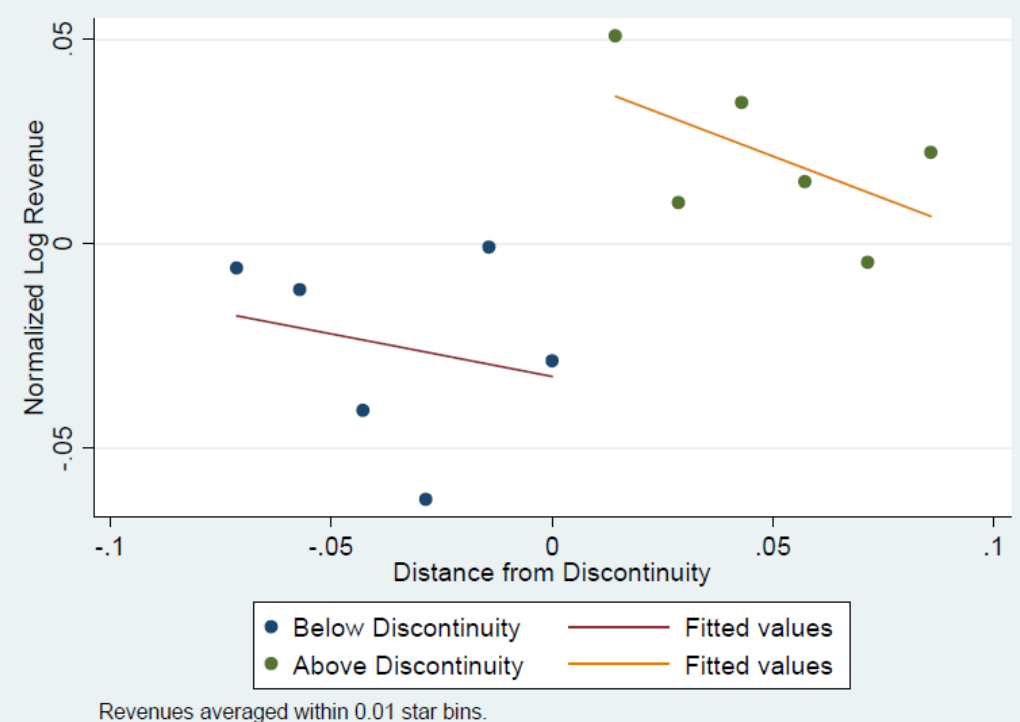
\includegraphics[width=0.3\textwidth]{figures/f4}
        \caption{ Yelp star ratings}
    \label{figure 4}
  \end{center}
\end{figure}

\subsection{Difference in Differences}
\subparagraph{Compare differences after a sudden change with trends in a control group} If minimum wage changes in one state, for example, the effect may be visible in the difference in the trend line, as shown in Firgure 5.

\begin{figure}[ht]
  \begin{center}
    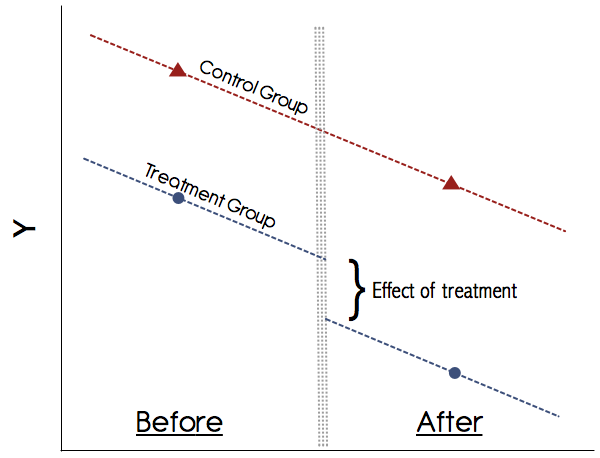
\includegraphics[width=0.3\textwidth]{figures/f5}
        \caption{Difference in Treatments can be seen in Trendlines}
    \label{figure 5}
  \end{center}
\end{figure}


\end{document}

\end{document}

%%% Local Variables:
%%% mode: latex
%%% TeX-master: t
%%% End:
